

\chapter{图表、公式格式和印制要求Abc}
\thispagestyle{others}
\pagestyle{others}

\section{本章引言}


\section{图和表格式}

图、表在版面中居中放置,图编号和图题居中列在图下。编号采用阿拉伯数字分章连续编号,例如“图 \ref{fig:3.1}”,“表 \ref{tab:3.1}”以及“式 \ref{eq:3.1}”。

\subsection{图}
下面给出图片示例:

%调整图片与上方文字之间的间距
\vspace{-0.15cm}

\begin{figure}[h]
		\centering 
		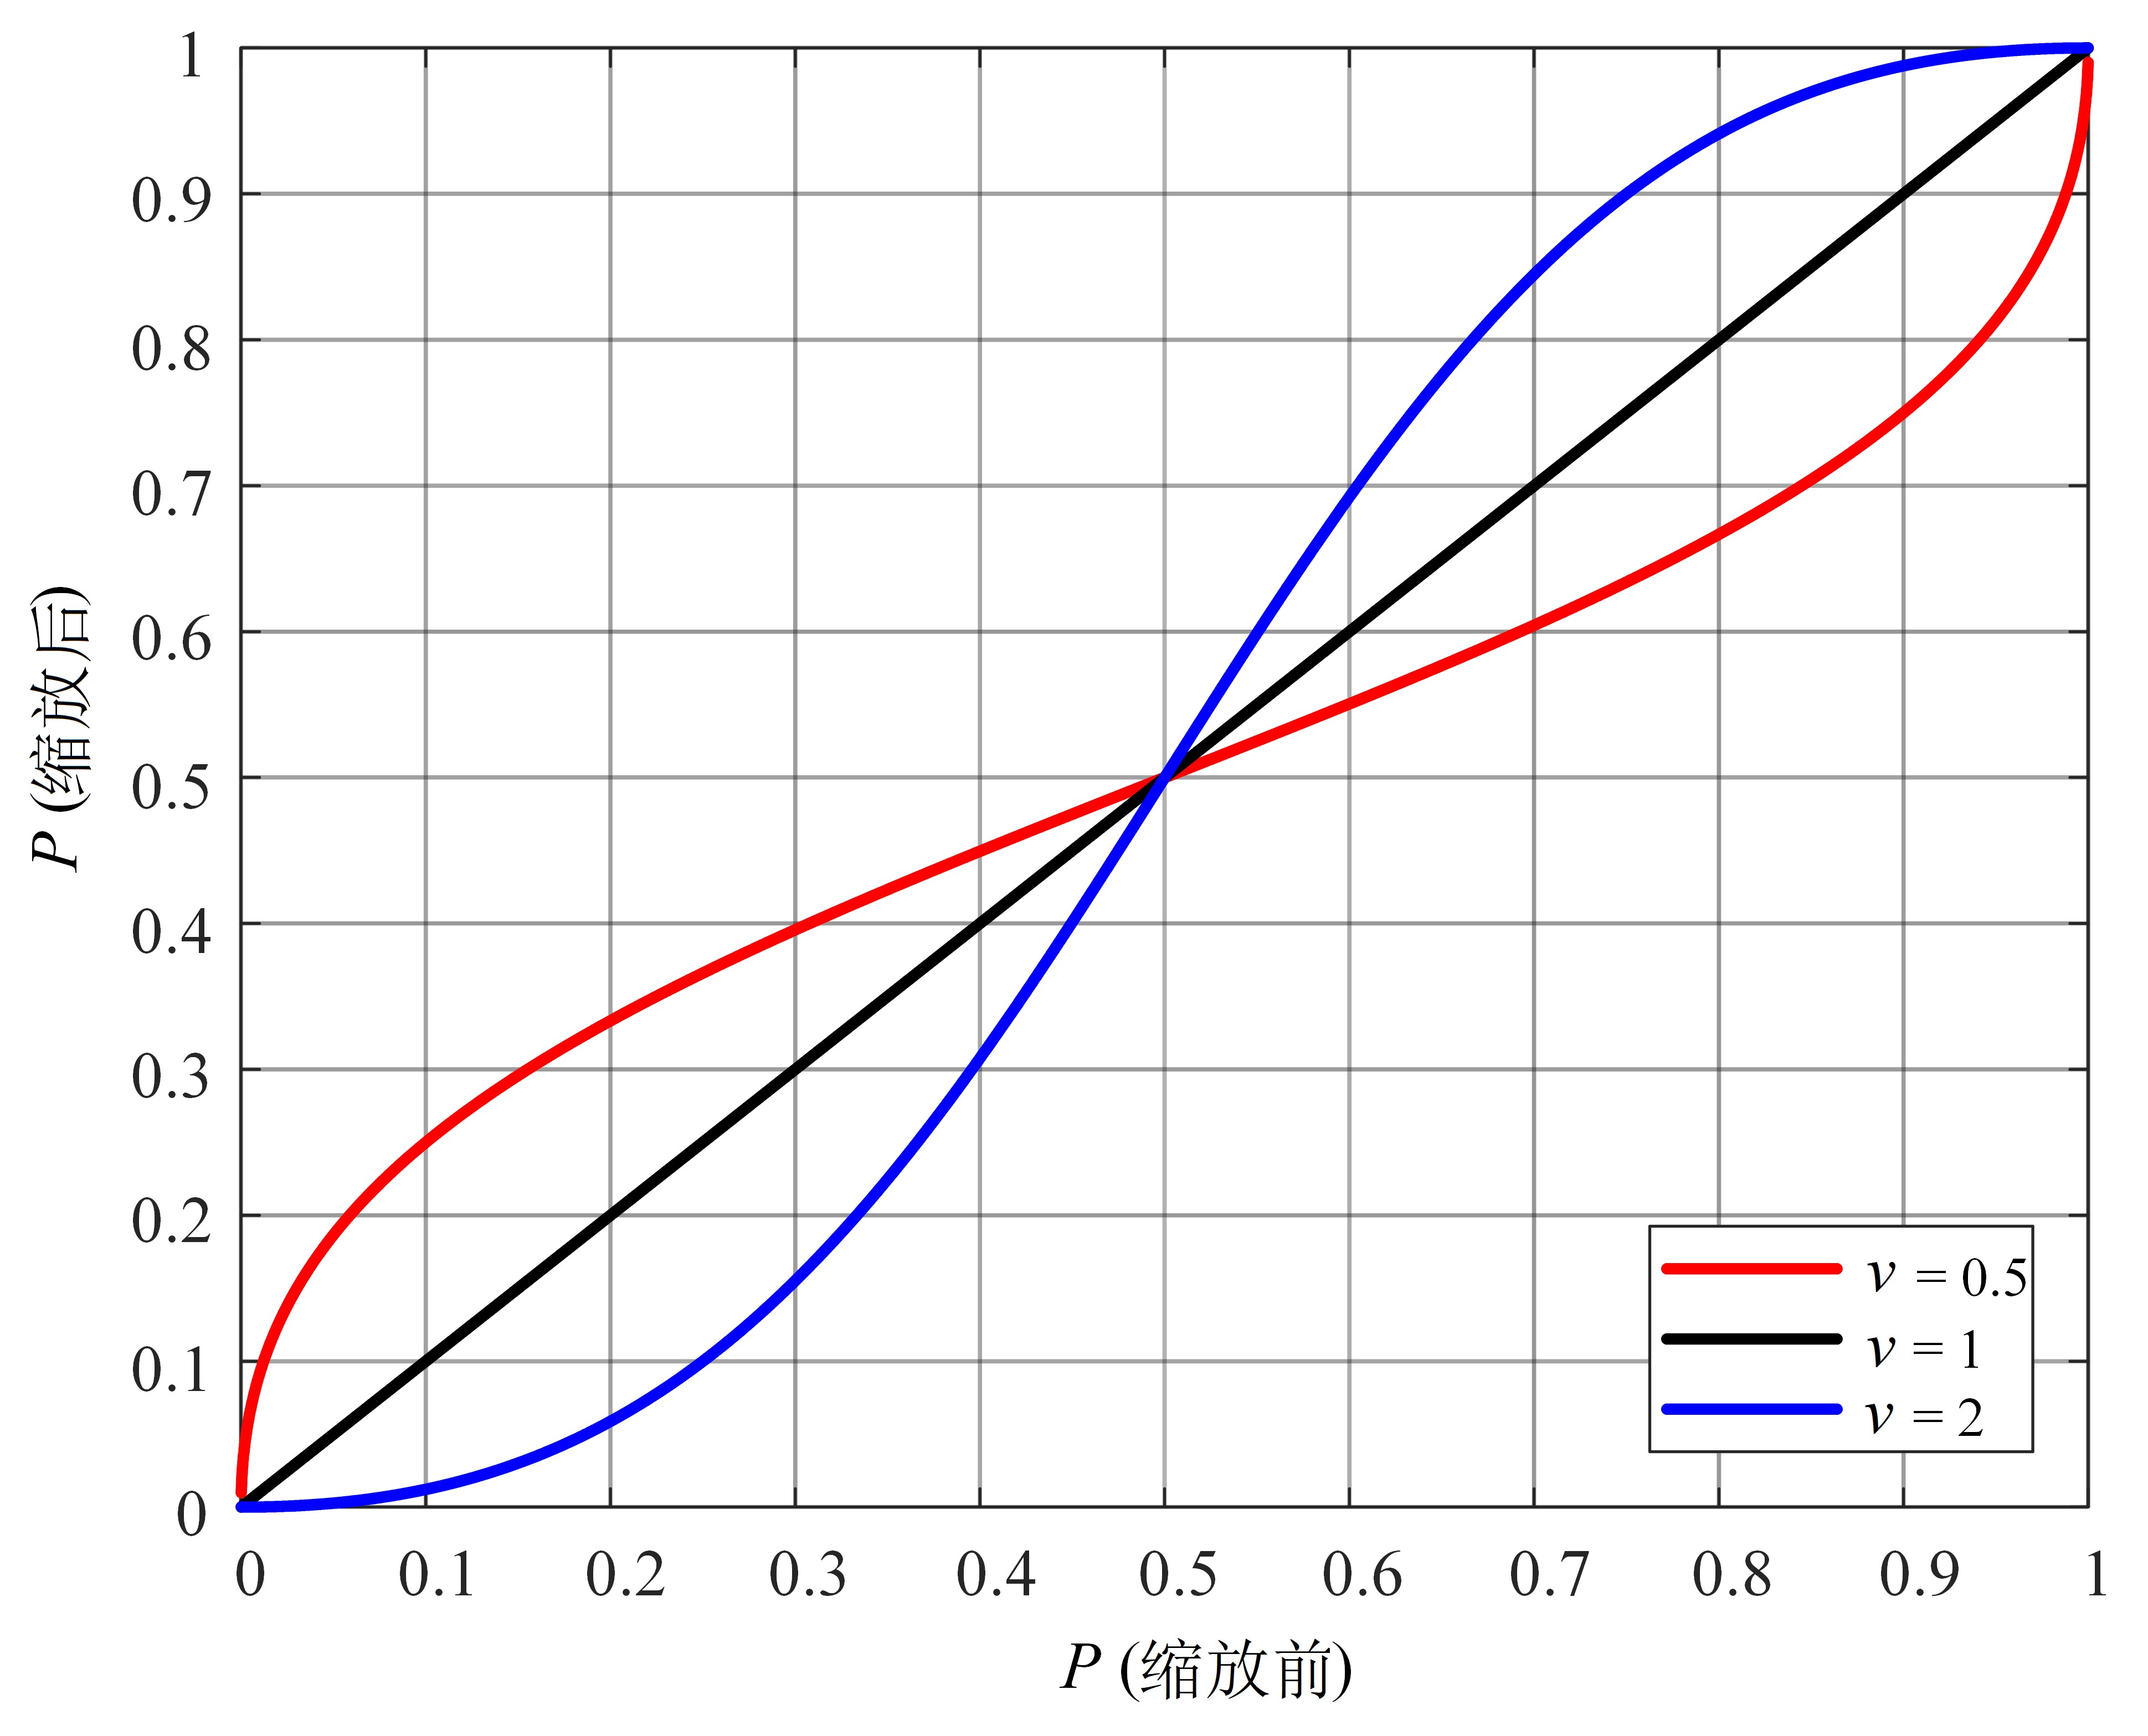
\includegraphics[width=10cm]{chapters/chapter3/31.jpg}
	    \bicaption[\xiaosi 不同缩放系数v的缩放效果]{\wuhao 不同缩放系数v的缩放结果}{\wuhao Scaling results with different scaling coefficients ν}
		\label{fig:3.1} 
\end{figure}

%调整图片与下方文字之间的间距
\vspace{-0.5cm}

图片标题的间距按照上述设置即可,与上下文的间距由于LATEX动态排版特性,需要大家手动调整。

。

。

。

。



下图是多子图示例:
%\vspace{-1cm}



\begin{figure}[h]
	\centering
	\subfigure[]{
		\label{fig:DE_J}
		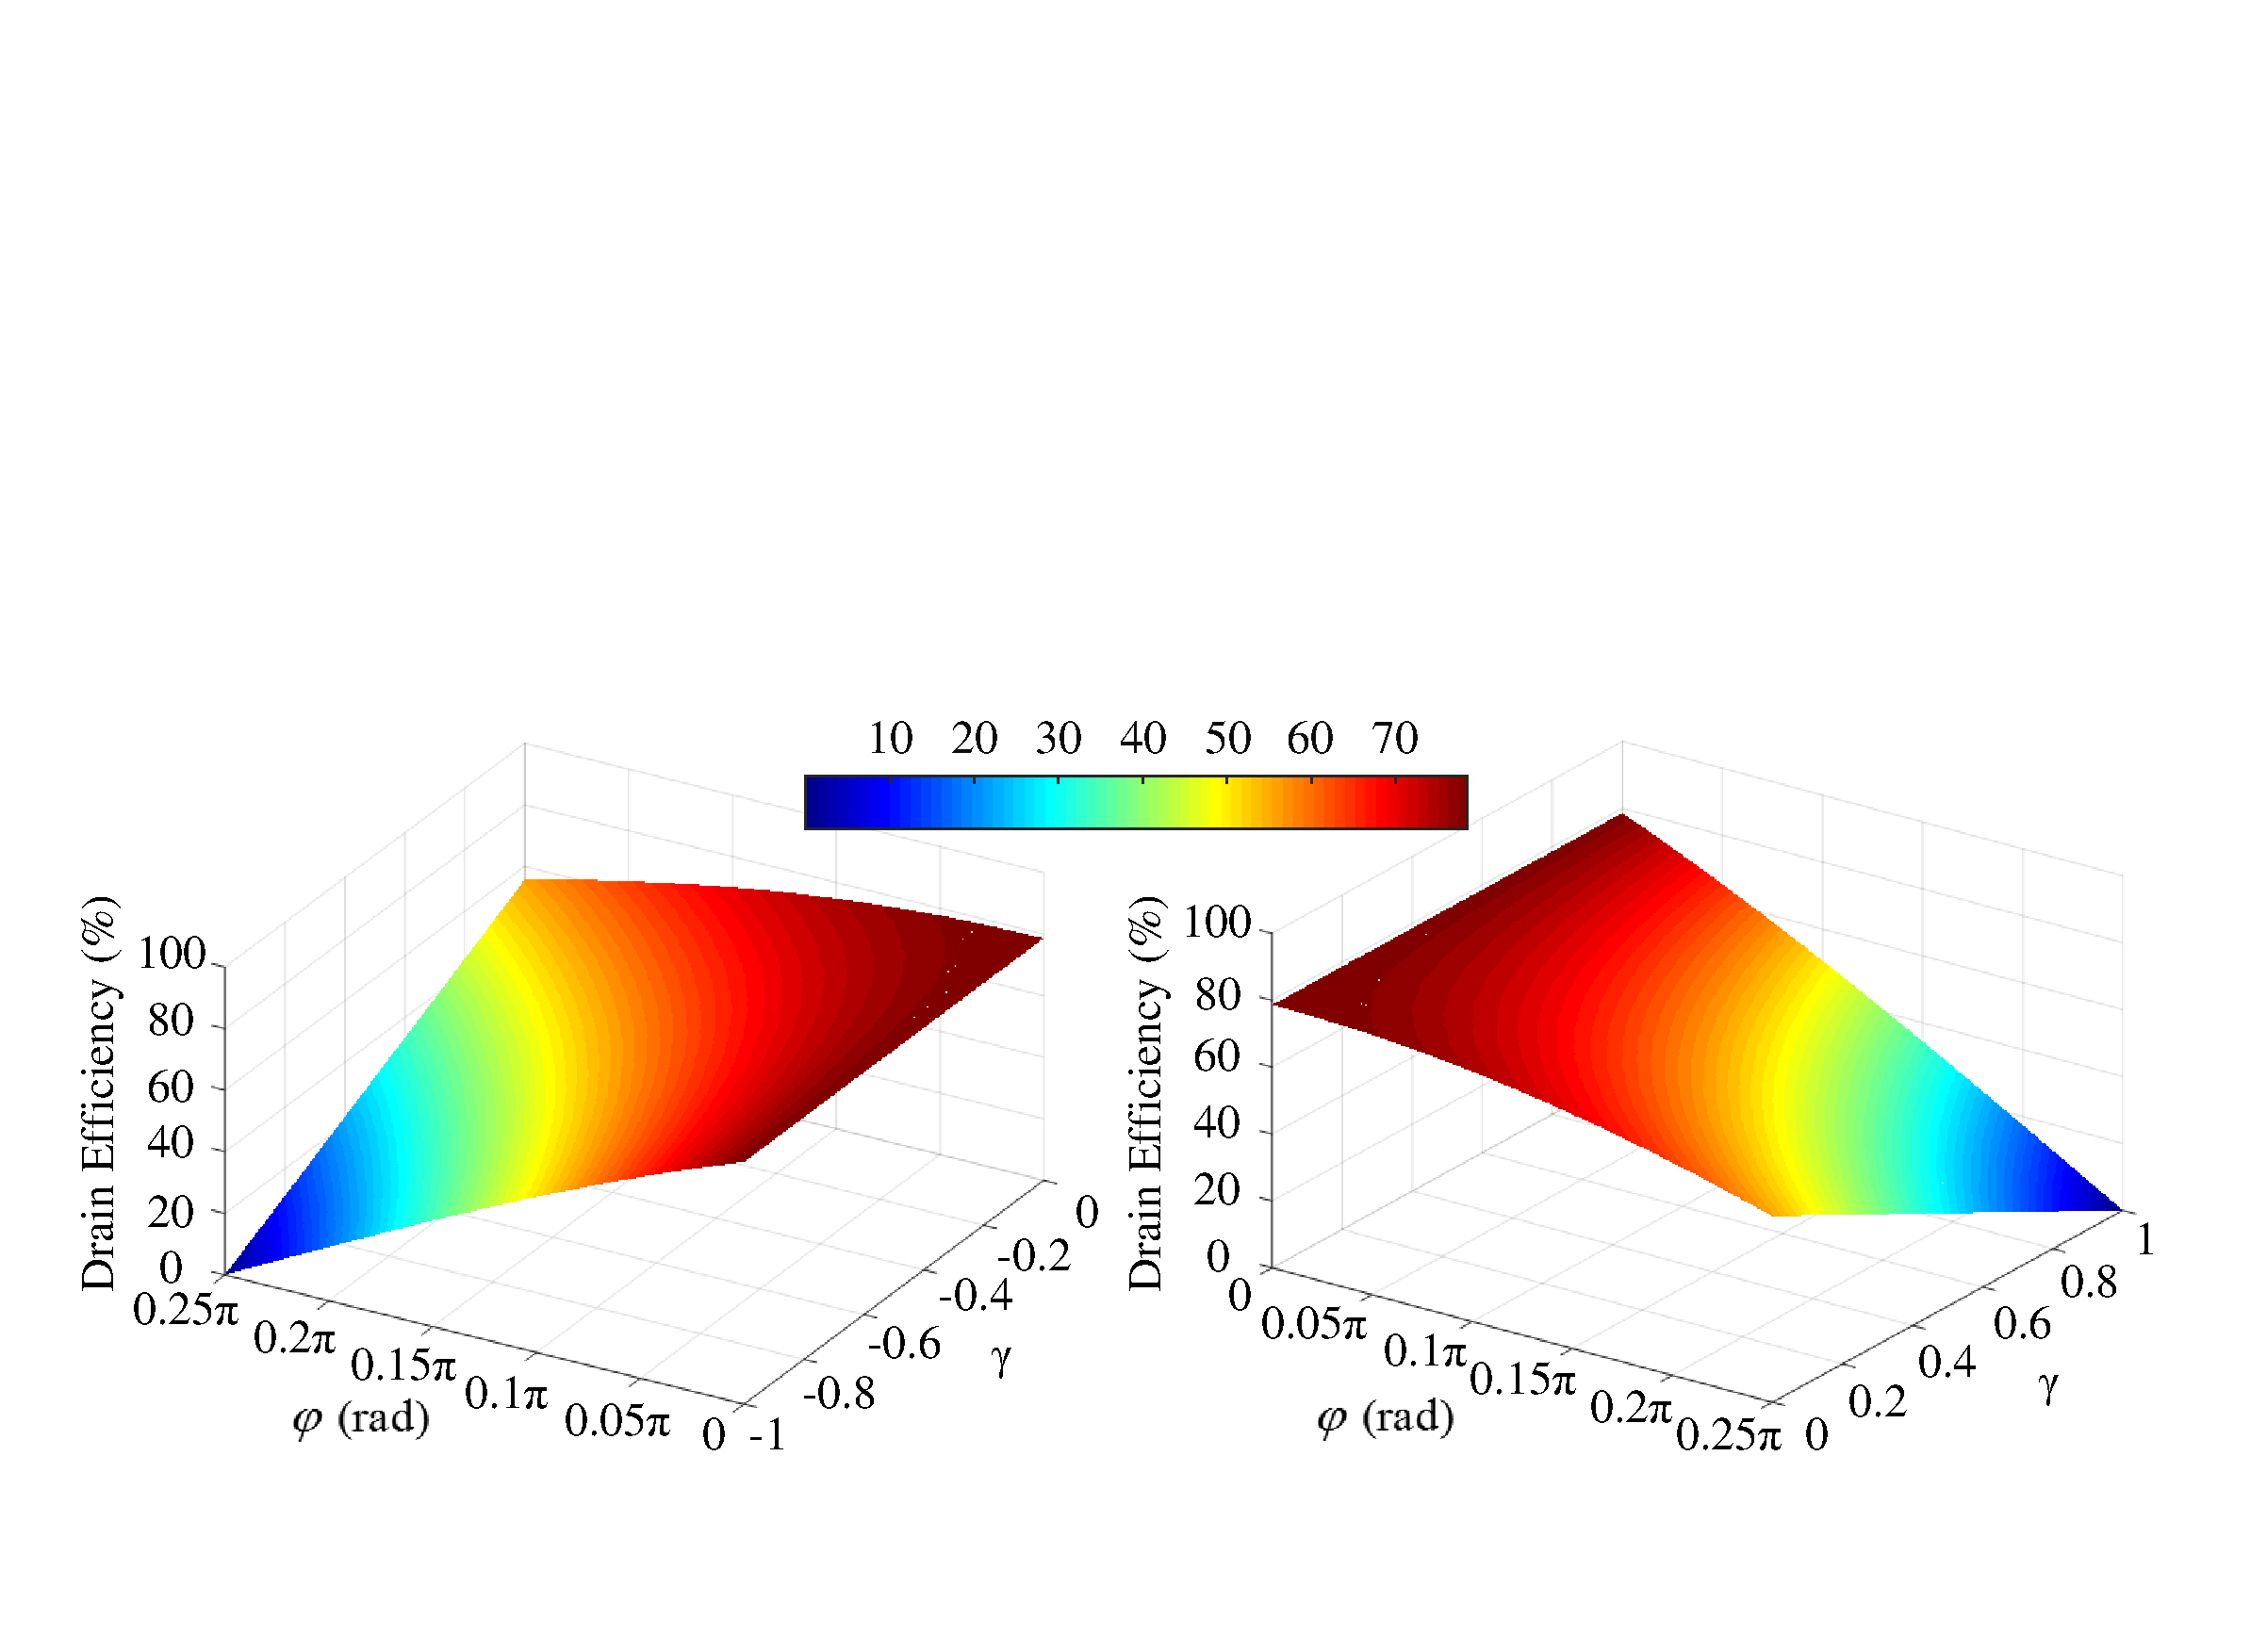
\includegraphics[width=12cm]{chapters/chapter3/DE_J.pdf}}
	\subfigure[]{
		\label{fig:DE_CF}
		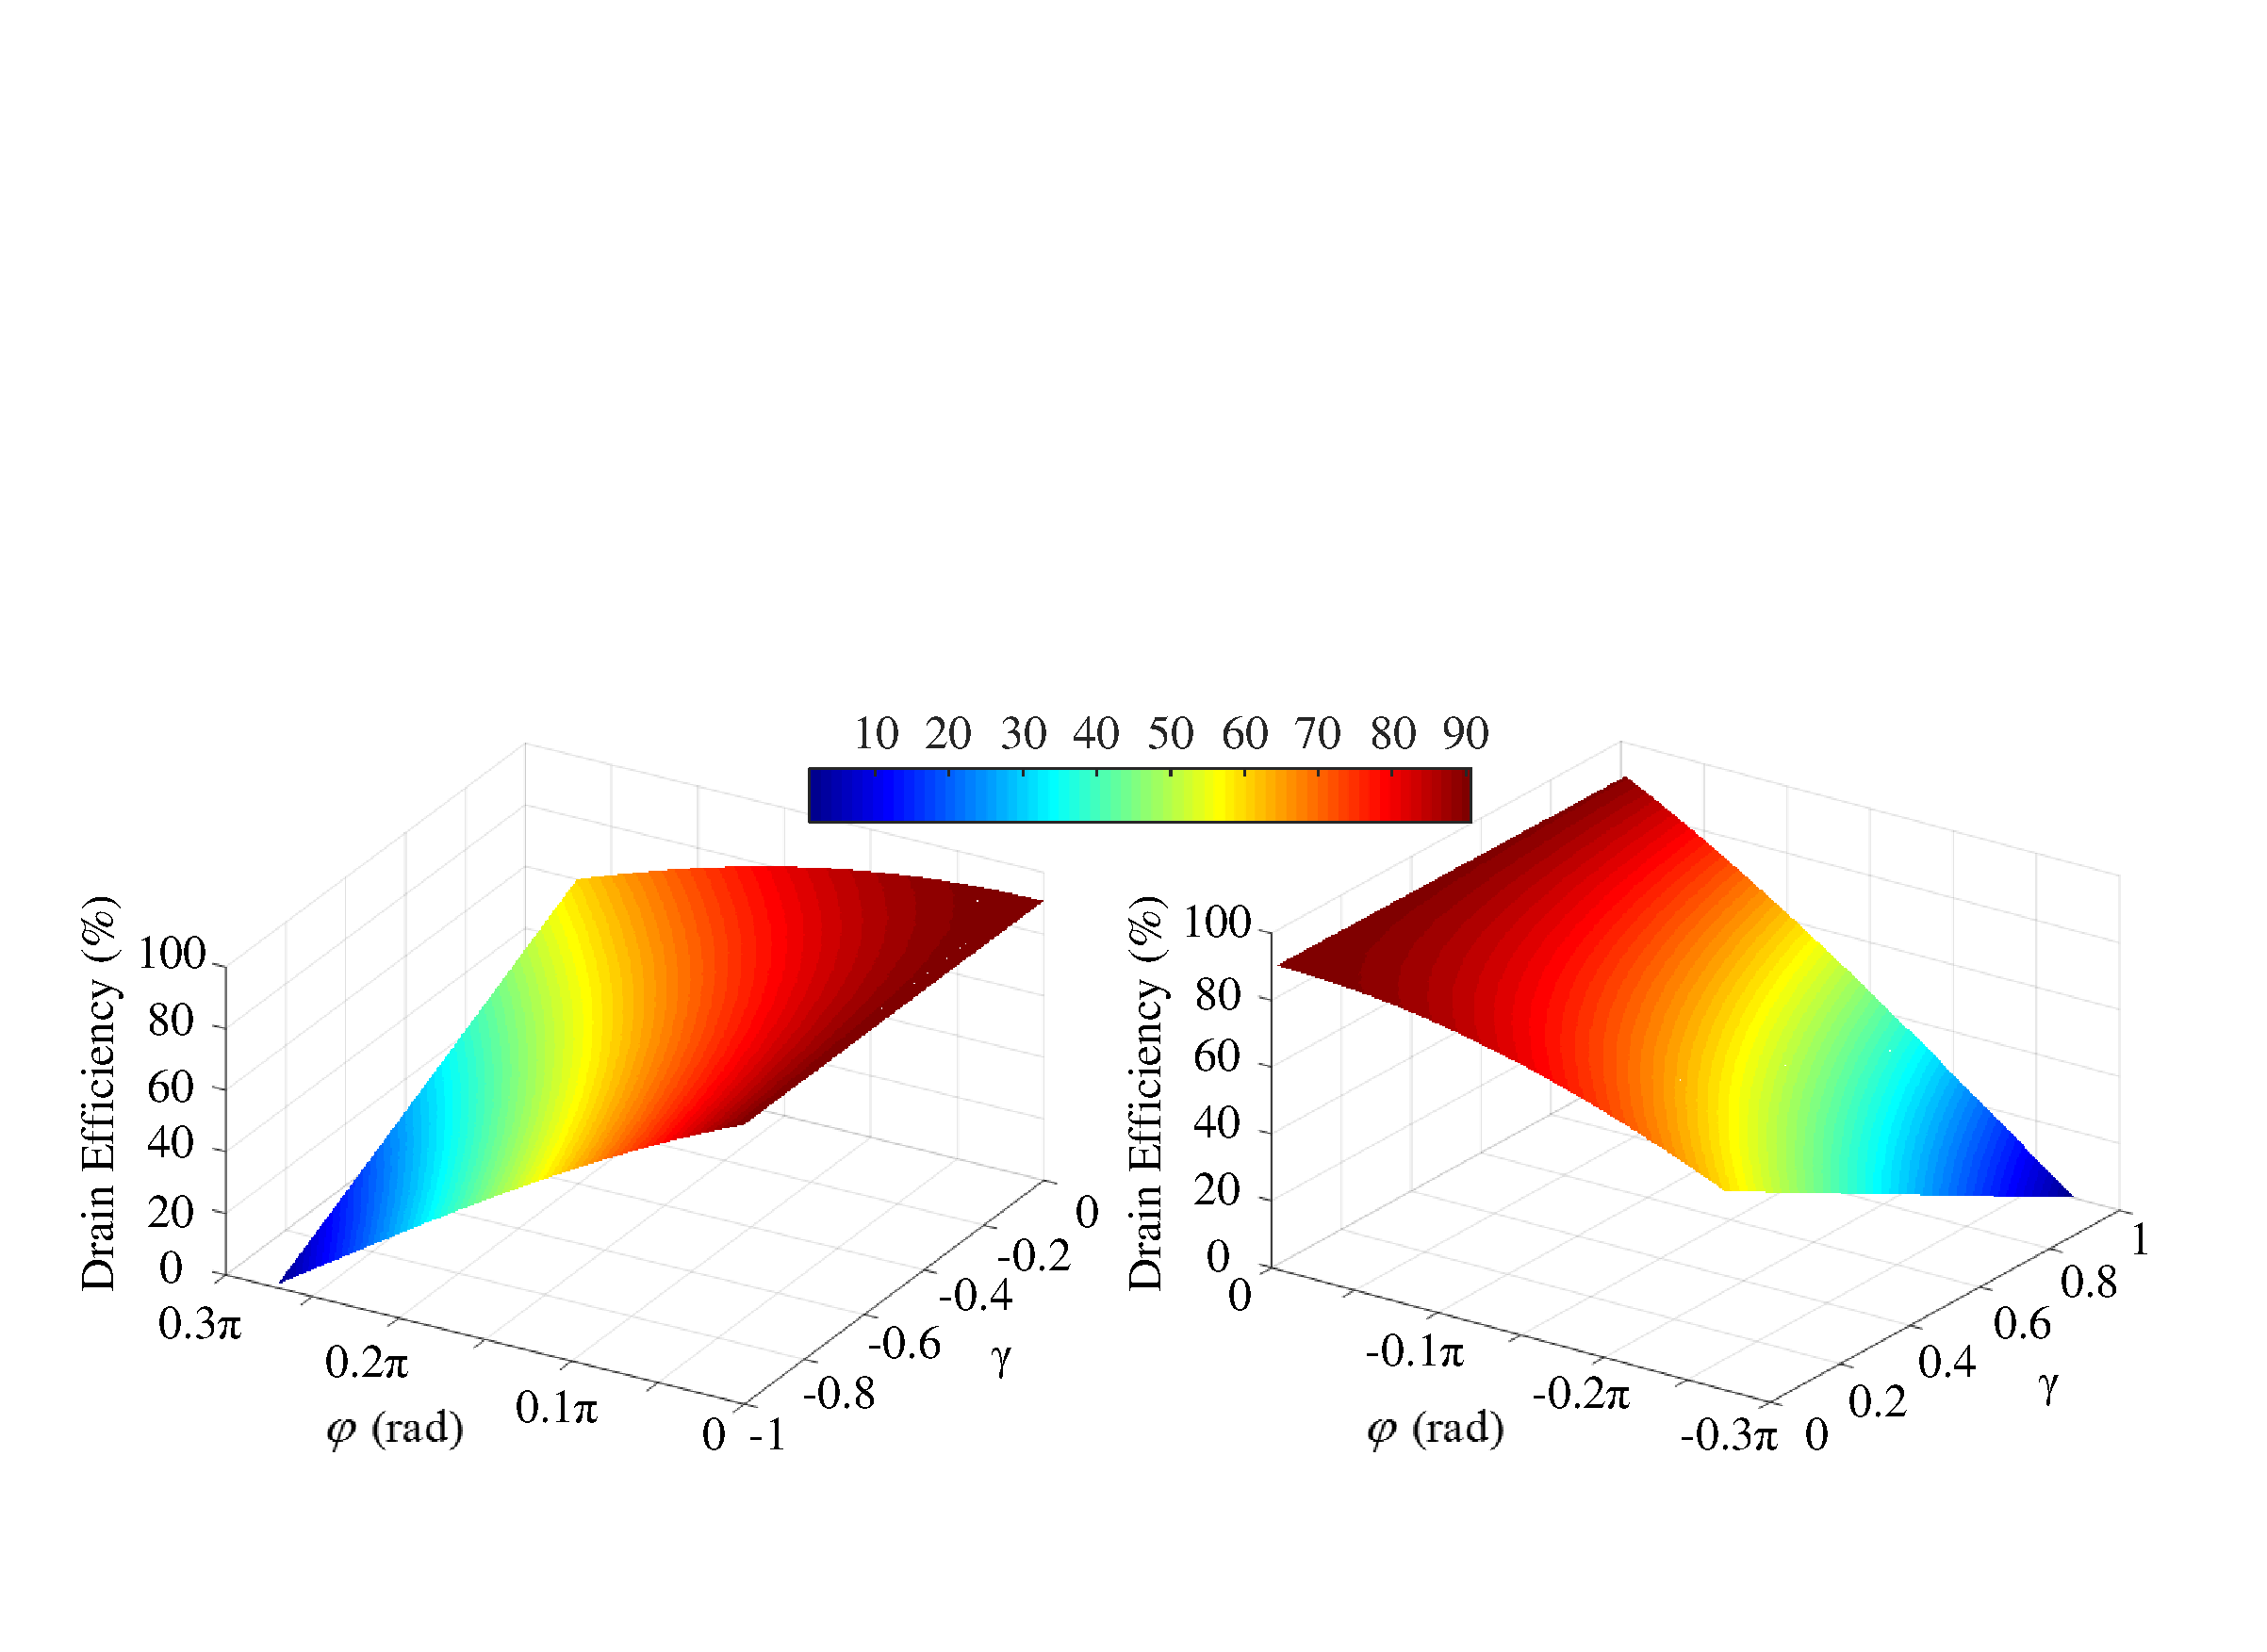
\includegraphics[width=12cm]{chapters/chapter3/DE_CF.pdf}}    
\bicaption[\xiaosi 理论效率与$\gamma$和$\varphi$的关系。]{\wuhao 理论效率与$\gamma$和$\varphi$的关系。 (a) $\alpha=1$; (b) $\alpha=2/\sqrt{3}$}{\wuhao Theoretical DE versus $\gamma$ and $\varphi$. (a) $\alpha=1$. (b) $\alpha=2/\sqrt{3}$}

%	\caption{\wuhao 理论效率与$\gamma$和$\varphi$的关系。 (a) $\alpha=1$; (b) $\alpha=2/\sqrt{3}$}
%%	\raggedright
%	\wuhao Fig. 3-2 Theoretical DE versus $\gamma$ and $\varphi$. (a) $\alpha=1$. (b) $\alpha=2/\sqrt{3}$.Theoretical DE versus $\gamma$ and $\varphi$. (a) $\alpha=1$. (b) $\alpha=2/\sqrt{3}$.
\end{figure}

\vspace{-0.5cm}

\subsection{表}

表格格式参照写作指南。表格格式参照写作指南。表格格式参照写作指南。表格格式参照写作指南。表格格式参照写作指南。表格格式参照写作指南。表格格式参照写作指南。表格格式参照写作指南。表格格式参照写作指南。表格格式参照写作指南。表格格式参照写作指南。表格格式参照写作指南。表格格式参照写作指南。表格格式参照写作指南。表格格式参照写作指南。表格格式参照写作指南。

\vspace{0.1cm}

\begin{table}[h]
	\renewcommand{\arraystretch}{1.5}
	\centering
	\bicaption[\xiaosi 电流类型对效率的影响]{\wuhao 电流类型对效率的影响}{\wuhao Current type impact on efficiency}
	\begin{tabular}{p{3cm}p{3cm}p{3cm}p{3cm}}
		\toprule[1.5pt]
		\makecell[c]{\songti\wuhao 电流类型}&\makecell[c]{\songti\wuhao A}&\makecell[c]{\songti\wuhao B}&\makecell[c]{\songti\wuhao C}\\
		\hline
		\makecell[c]{\wuhao aaa}&\makecell[c]{\wuhao aa1}&\makecell[c]{\wuhao bb1}&\makecell[c]{\wuhao cc1}\\
		\bottomrule[1.5pt]
	\end{tabular}
   \label{tab:3.1} 
\end{table}

表格格式参照写作指南。表格格式参照写作指南。表格格式参照写作指南。表格格式参照写作指南。表格格式参照写作指南。表格格式参照写作指南。表格格式参照写作指南。表格格式参照写作指南。表格格式参照写作指南。表格格式参照写作指南。表格格式参照写作指南。表格格式参照写作指南。表格格式参照写作指南。表格格式参照写作指南。表格格式参照写作指南。表格格式参照写作指南。

%\vspace{-0.8cm}

\begin{table*}[h]
	\renewcommand{\arraystretch}{1.5}
	\bicaption[\xiaosi 高效率功放性能对比]{\wuhao 高效率功放性能对比}{\wuhao High-effiency power amplifier performance comparison}
	\label{tab_1}
	\centering
	\wuhao
	\begin{tabular}{c c c c c }
		\hline
		{\textbf{带宽}(GHz)}&{\textbf{功率}(dBm)}&{\textbf{效率}(\%)}&{\textbf{线性度}(dBc)}&{\textbf{信号带宽}(MHz)}\\
		\hline
		1.4--2.6&32--34&30--40 (DE)&-25 -- -30 (ACLR)&5\\
		\hline
		\multirow{2}{*}{2.1--2.7}&39&45 (DE) @ 2.14 GHz&--31 (ACLR)&\multirow{2}{*}{5}\\\cline{3-4}
		&(average)&40 (DE) @ 2.655 GHz&--30 (ACLR)&\\
		\hline
		3.5&38.1&59 (PAE)&30 (C/I)&5\\
		\hline
		\multirow{2}{*}{1.6--2.6}&36.0--38.5&45--60 (PAE)&30 (C/I)&5\\\cline{2-5}
		&35.3--37.5&40--55 (PAE)&--30 (ACLR)&20\\
		\hline
	\end{tabular}
\end{table*}

%\begin{longtable}{lcccccccccc}
%%	\small
%	\renewcommand{\arraystretch}{1.25}
%%	\centering
%%		\toprule[1.5pt]
%%	\caption{\wuhao 标签噪声对各对比算法约简结果的影响}\\
%%	\label{tab:4-9}\\
%%	\toprule[1.5pt]	
%    \hline
%	\multirow{2}{*}{数据集} & \multicolumn{1}{c}{ILFS}      & \multicolumn{1}{c}{mRMR} & \multicolumn{1}{c}{GBNRS}   & \multicolumn{2}{c}{NRS}& \multicolumn{2}{c}{WNRS} & \multicolumn{3}{c}{FGBRS}         \\ \cline{2-11}
%	\multicolumn{1}{c}{} &精度  & 精度 &精度  & $O\delta$  & 精度   & $O\delta$ & 精度     & $O\delta$ & $OP_T$  & 精度   \\ \hline
% 
%	\endfirsthead  %第一页表头内容
%	
%%	\toprule[1.5pt]
%\hline
%	\multirow{2}{*}{数据集} & \multicolumn{1}{c}{ILFS}      & \multicolumn{1}{c}{mRMR} & \multicolumn{1}{c}{GBNRS}   & \multicolumn{2}{c}{NRS}& \multicolumn{2}{c}{WNRS} & \multicolumn{3}{c}{FGBRS}         \\ \cline{2-11}
%	\multicolumn{1}{c}{} &精度  & 精度 &精度  & $O\delta$  & 精度   & $O\delta$ & 精度     & $O\delta$ & $OP_T$  & 精度   \\ \hline
%	\endhead  %每一页表头内容
%	
%	\hline
%	\endfoot
%	
%	\hline
%	\endlastfoot
%	
%	Wine(0\%)            & 0.9776   & 0.9776   & 0.9438   & 0.22     & 0.9829       & 0.24      & 0.9717       & 0.10   & 0.92   & 1.0000    \\
%	Wine(5\%)            & 0.9044   & 0.9048   & 0.9606   & 0.14     & 0.9610       & 0.12      & 0.9497       & 0.02   & 0.92   & 0.9722    \\
%	Wine(15\%)           & 0.7695   & 0.7690   & 0.8817   & 0.18     & 0.8935       & 0.18      & 0.8768       & 0.02   & 0.92   & 0.9722    \\
%	Wine(25\%)           & 0.5957   & 0.6005   & 0.7524   & 0.14     & 0.7643       & 0.20      & 0.7586       & 0.16   & 0.96   & 0.8611    \\
%	Wine(35\%)           & 0.5390   & 0.5843   & 0.5343   & 0.18     & 0.5790       & 0.12      & 0.5957       & 0.02   & 0.98   & 0.8056    \\
%	Pima(0\%)            & 0.7322   & 0.7358   & 0.7331   & 0.08     & 0.7435       & 0.06      & 0.7435       & 0.10   & 0.98   & 0.7597    \\
%	Pima(5\%)            & 0.7223   & 0.7126   & 0.7084   & 0.02     & 0.6953       & 0.08      & 0.6875       & 0.06   & 0.96   & 0.7468    \\
%	Pima(15\%)           & 0.6679   & 0.6796   & 0.6184   & 0.02     & 0.6262       & 0.06      & 0.6250       & 0.02   & 0.80   & 0.7338    \\
%	Pima(25\%)           & 0.5598   & 0.5780   & 0.5457   & 0.06     & 0.5546       & 0.04      & 0.5546       & 0.02   & 0.96   & 0.6558    \\
%	Pima(35\%)           & 0.5104   & 0.5156   & 0.5247   & 0.02     & 0.5455       & 0.02      & 0.5442       & 0.08   & 0.78   & 0.5909    \\
%	Cancer(0\%)          & 0.9634   & 0.9678   & 0.9678   & 0.26     & 0.9722       & 0.24      & 0.9765       & 0.20   & 0.98   & 0.9708    \\
%	Cancer(5\%)          & 0.9267   & 0.9252   & 0.9195   & 0.02     & 0.9151       & 0.10      & 0.9239       & 0.02   & 0.98   & 0.9708    \\
%	Cancer(15\%)         & 0.7697   & 0.7756   & 0.7541   & 0.02     & 0.7555       & 0.02      & 0.7628       & 0.12   & 0.76   & 0.8394    \\
%	Cancer(25\%)         & 0.6144   & 0.6012   & 0.5828   & 0.02     & 0.5652       & 0.04      & 0.5667       & 0.20   & 0.72   & 0.6569    \\
%	Cancer(35\%)         & 0.5131   & 0.5131   & 0.4963   & 0.02     & 0.5300       & 0.04      & 0.5388       & 0.02   & 0.74   & 0.6667    \\
%	Diabetes(0\%)        & 0.7432   & 0.7510   & 0.7291   & 0.06     & 0.7461       & 0.06      & 0.7435       & 0.02   & 0.92   & 0.7922    \\
%	Diabetes(5\%)        & 0.5476   & 0.5918   & 0.7161   & 0.02     & 0.7240       & 0.02      & 0.7240       & 0.12   & 0.90   & 0.7857    \\
%	Diabetes(15\%)       & 0.5658   & 0.5906   & 0.5951   & 0.02     & 0.6107       & 0.04      & 0.6211       & 0.04   & 0.90   & 0.7532    \\
%	Diabetes(25\%)       & 0.5215   & 0.5334   & 0.5117   & 0.04     & 0.5522       & 0.04      & 0.5521       & 0.12   & 0.78   & 0.7013    \\
%	Diabetes(35\%)       & 0.5476   & 0.5020   & 0.5079   & 0.06     & 0.5287       & 0.08      & 0.5287       & 0.02   & 0.92   & 0.5844    \\
%	Haberman(0\%)        & 0.6894   & 0.6703   & 0.7091   & 0.06     & 0.6929       & 0.02      & 0.6896       & 0.02   & 0.82   & 0.7581    \\
%	Haberman(5\%)        & 0.7681   & 0.6829   & 0.6567   & 0.02     & 0.6567       & 0.02      & 0.6567       & 0.02   & 0.80   & 0.7419    \\
%	Haberman(15\%)       & 0.6141   & 0.5816   & 0.6048   & 0.02     & 0.6405       & 0.02      & 0.6307       & 0.02   & 0.98   & 0.6774    \\
%	Haberman(25\%)       & 0.4932   & 0.5653   & 0.4669   & 0.02     & 0.5262       & 0.02      & 0.5196       & 0.02   & 0.76   & 0.6613    \\
%	Haberman(35\%)       & 0.4611   & 0.5556   & 0.4769   & 0.02     & 0.5358       & 0.04      & 0.5391       & 0.02   & 0.88   & 0.5968    \\
%	Horse(0\%)           & 0.8017   & 0.8152   & 0.8126   & 0.26     & 0.7966       & 0.28      & 0.8020       & 0.06   & 0.80   & 0.8649    \\
%	Horse(5\%)           & 0.7719   & 0.7610   & 0.7772   & 0.02     & 0.7854       & 0.20      & 0.7799       & 0.20   & 0.76   & 0.8649    \\
%	Horse(15\%)          & 0.6413   & 0.6275   & 0.6576   & 0.26     & 0.6903       & 0.12      & 0.7036       & 0.26   & 0.76   & 0.8514    \\
%	Horse(25\%)          & 0.6330   & 0.6384   & 0.5407   & 0.20     & 0.5436       & 0.14      & 0.5762       & 0.28   & 0.98   & 0.8108    \\
%	Horse(35\%)          & 0.4866   & 0.5188   & 0.5056   & 0.06     & 0.4754       & 0.14      & 0.5352       & 0.26   & 0.86   & 0.7027    \\
%	Sonar(0\%)           & 0.8226   & 0.8367   & 0.7738   & 0.24     & 0.8226       & 0.24      & 0.8170       & 0.28   & 0.88   & 0.9286    \\
%	Sonar(5\%)           & 0.5000   & 0.5575   & 0.7268   & 0.20     & 0.7596       & 0.20      & 0.7598       & 0.24   & 0.88   & 0.9048    \\
%	Sonar(15\%)          & 0.5671   & 0.5722   & 0.6204   & 0.06     & 0.6966       & 0.28      & 0.6879       & 0.14   & 0.98   & 0.8810    \\
%	Sonar(25\%)          & 0.4756   & 0.5089   & 0.4765   & 0.20     & 0.6005       & 0.22      & 0.6157       & 0.26   & 0.98   & 0.7619    \\
%	Sonar(35\%)          & 0.5098   & 0.5146   & 0.5823   & 0.18     & 0.5519       & 0.12      & 0.5919       & 0.24   & 0.90   & 0.7143    \\
%	WDBC(0\%)            & 0.9666   & 0.9719   & 0.9631   & 0.10     & 0.9683       & 0.26      & 0.9630       & 0.12   & 0.98   & 0.9912    \\
%	WDBC(5\%)            & 0.8840   & 0.8840   & 0.8964   & 0.28     & 0.9261       & 0.26      & 0.9209       & 0.14   & 0.98   & 0.9912    \\
%	WDBC(15\%)           & 0.7311   & 0.7294   & 0.7733   & 0.16     & 0.7750       & 0.18      & 0.7645       & 0.08   & 0.82   & 0.9737    \\
%	WDBC(25\%)           & 0.6169   & 0.594    & 0.5783   & 0.06     & 0.5869       & 0.02      & 0.5834       & 0.02   & 0.72   & 0.8246    \\
%	WDBC(35\%)           & 0.4939   & 0.5062   & 0.4728   & 0.08     & 0.5219       & 0.22      & 0.5326       & 0.02   & 0.72   & 0.6667    \\
%	Heart1(0\%)          & 0.7582   & 0.7649   & 0.7485   & 0.20     & 0.7416       & 0.08      & 0.7383       & 0.26   & 0.92   & 0.8305    \\
%	Heart1(5\%)          & 0.7281   & 0.7652   & 0.7314   & 0.04     & 0.7553       & 0.08      & 0.7857       & 0.28   & 0.90   & 0.8475    \\
%	Heart1(15\%)         & 0.6428   & 0.6462   & 0.6499   & 0.08     & 0.6463       & 0.08      & 0.6700       & 0.18   & 0.88   & 0.7966    \\
%	Heart1(25\%)         & 0.5067   & 0.5168   & 0.5750   & 0.06     & 0.5815       & 0.12      & 0.5746       & 0.14   & 0.82   & 0.7627    \\
%	Heart1(35\%)         & 0.4864   & 0.5137   & 0.5241   & 0.02     & 0.5444       & 0.10      & 0.5307       & 0.14   & 0.76   & 0.6779    \\
%	Average              & 0.6609   & 0.6691   & 0.6730   & -        & 0.6904       & -         & 0.6936       & -      & -      & 0.7978 \\	
%%	\toprule[1.5pt]  
%\end{longtable} 


\section{公式格式}

\begin{equation}
\left\{ \begin{aligned}
0.794 \le \zeta  \le 1 ~~~~~~~~~~~\\
0.631 \le \gamma  = \frac{{0.631}}{{{\zeta ^2}}} \le 1~~~~~~ \\
- \frac{1}{{2\gamma }} \le \delta  \le \frac{1}{{2\gamma }}~~~~~~~~~~~ \\
{Z_{c,low,f}} = 2{R_{opt}}(\gamma  + j\delta )~~~~~\\
{Z_{c,2f}} = {Z_{c,low,2f}} =  - j\frac{{3\pi }}{4}\gamma \delta {R_{opt}}
\end{aligned} \right.
\label{eq:3.1}
\end{equation}

\begin{equation}
\begin{aligned}
v(\theta ) = V_{DD}\cdot(1 - \alpha cos(\theta  + \varphi ) + \beta cos(3\theta  + 3\varphi ))\\
\cdot(1 - \gamma \sin (\theta  + \varphi )) ~~~~~- 1 \le \gamma  \le 1\
\end{aligned}
\label{eq:vd}
\end{equation}




\noindent
公式格式测试。中文摘要及之后的前置部分,包括中文摘要、ABSTRACT、目录、图目录(如有)、表目录(如有)、主要符号表(如有)、缩略词表(如有),在双面印刷时,若某部分页数为奇数,则该部分最后一页单面印刷。

\section{印制要求}
涉密学位论文的印刷、制作、传递、存档等,须符合国家、学校相关保密要求。学位论文一律左侧装订。

中文摘要之前的前置部分(封面、中、英文题名页、独创性声明和使用授权书),采用单面印刷。

从中文摘要开始,采用双面印刷。

中文摘要及之后的前置部分,包括中文摘要、ABSTRACT、目录、图目录(如有)、表目录(如有)、主要符号表(如有)、缩略词表(如有),在双面印刷时,若某部分页数为奇数,则该部分最后一页单面印刷。例如:若“摘要”只有1页,则其页码是“Ⅰ”,第“Ⅰ”页纸的背面为空白(无页眉或页码);“ABSTRACT”用新的一张纸印刷,页码从“Ⅱ”开始。

从第1章第1页开始,至论文最后1页,所有页面均双面印刷。例如:若第1章的最后1页为第17页,则第2章的第1页在第17页的背面印刷,页码为“18”(页眉是“重庆邮电大学博士(硕士)学位论文”)。

一次性双面打印整本学位论文技巧:除用于打印的版本外,电子版论文中一律不得出现空白页。论文打印建议使用PDF格式。为方便一次性双面打印,有时可在单面印刷的部分(如封面、中、英文题名页、独创性声明和使用授权书),或者双面打印只有1页的某部分内容(如摘要、ABSTRACT等)后插入1页空白页,该空白页不编排页眉页码;论文中出现的页码应前后连续,不得中断。

\subsection{算法流程}
	算法由标题、输入、输出组成,如算法\ref{algo1}所示。

\begin{algorithm}[htb]
	%	\renewcommand{\algorithmicrequire}{\textbf{Input:}}
	%	\renewcommand{\algorithmicensure}{\textbf{Output:}}
		\caption{xxx的算法流程}\label{algo1}
		\setlength{\baselineskip}{18bp}
		\begin{algorithmic}[1]
			\Require {原始图像: $ X $; 目标图像: $ Y $;;小批量数据采样器: $ SA $; 批次大小: $ k $; 学习率:$ lr $。}
			\Ensure {$G$,参数为$ \theta $。}
			\State \textbf{初始化:} $G$的参数为$\theta$。
			\While {$ \theta_1 $未收敛}
			\State $ x\gets y $ \{注释注释注释注释注释注释\};
			\State $ x\gets y $ \{注释注释注释注释注释注释\};
			\State $ x\gets y $ \{注释注释注释注释注释注释\};
			\State $ x\gets y $ \{注释注释注释注释注释注释\};
			\State $ x\gets y $ \{注释注释注释注释注释注释\};
			\State $ x\gets y $ \{注释注释注释注释注释注释\};
			\State $ x\gets y $ \{注释注释注释注释注释注释\};
			\State $ x\gets y $ \{注释注释注释注释注释注释\};
			\State $ x\gets y $ \{注释注释注释注释注释注释\};
			\State $ x\gets y $ \{注释注释注释注释注释注释\};
			\State $ x\gets y $ \{注释注释注释注释注释注释\};
			\State $ x\gets y $ \{注释注释注释注释注释注释\};
			\State $ x\gets y $ \{注释注释注释注释注释注释\};
			\State $ x\gets y $ \{注释注释注释注释注释注释\};
			\State $ x\gets y $ \{注释注释注释注释注释注释\};
			\State $ x\gets y $ \{注释注释注释注释注释注释\};
			\State $ x\gets y $ \{注释注释注释注释注释注释\};
			\EndWhile
		\end{algorithmic}
	\end{algorithm}

\section{本章小结}
本章介绍了……